
%% The first command in your LaTeX source must be the \documentclass command.
\documentclass[sigplan,screen,9pt]{acmart}
\settopmatter{printfolios=true,printccs=false,printacmref=false}

%%
%% \BibTeX command to typeset BibTeX logo in the docs
\AtBeginDocument{%
  \providecommand\BibTeX{{%
    \normalfont B\kern-0.5em{\scshape i\kern-0.25em b}\kern-0.8em\TeX}}}

%% Rights management information.  This information is sent to you
%% when you complete the rights form.  These commands have SAMPLE
%% values in them; it is your responsibility as an author to replace
%% the commands and values with those provided to you when you
%% complete the rights form.
\setcopyright{none}

%% These commands are for a PROCEEDINGS abstract or paper.
\acmConference[SE4AI WiSe'21]{Software Engineering for Artificial Intelligence}{Winter Semester 2021}{Darmstadt, Germany}
\acmYear{2021}
\acmBooktitle{}
\acmPrice{}
\acmISBN{}
\acmDOI{}


%%
%% Submission ID.
%% Use this when submitting an article to a sponsored event. You'll
%% receive a unique submission ID from the organizers
%% of the event, and this ID should be used as the parameter to this command.
%%\acmSubmissionID{123-A56-BU3}

%%
%% The majority of ACM publications use numbered citations and
%% references.  The command \citestyle{authoryear} switches to the
%% "author year" style.
%%
%% If you are preparing content for an event
%% sponsored by ACM SIGGRAPH, you must use the "author year" style of
%% citations and references.
%% Uncommenting
%% the next command will enable that style.
%%\citestyle{acmauthoryear}

%%
%% end of the preamble, start of the body of the document source.
\begin{document}

%%
%% The "title" command has an optional parameter,
%% allowing the author to define a "short title" to be used in page headers.
\title{Towards Intelligent Error Prediction and Rectification in IDEs}

%%
%% The "author" command and its associated commands are used to define
%% the authors and their affiliations.
%% Of note is the shared affiliation of the first two authors, and the
%% "authornote" and "authornotemark" commands
%% used to denote shared contribution to the research.
\author{Pritish Kishore Kumar}
%\affiliation

% Add additional authors by repeating the \author{} command like in the following
%\author{Max Musterfrau}
%\affiliation

%%
%% By default, the full list of authors will be used in the page
%% headers. Often, this list is too long, and will overlap
%% other information printed in the page headers. This command allows
%% the author to define a more concise list
%% of authors' names for this purpose.
%\renewcommand{\shortauthors}{Mustermann and Musterfrau}

%%
%% The abstract is a short summary of the work to be presented in the
%% article.
% No abstract for SE4AI summaries
%\begin{abstract}
%	Abstract
%\end{abstract}

%%
%% This command processes the author and affiliation and title
%% information and builds the first part of the formatted document.
\maketitle

\section{Introduction}
Code prediction is a technology that is primarily used in autocomplete techniques in intelligent Integrated Development Environments (IDEs). Popular IDEs are language-specific offerings from JetBrains such as IntelliJ (Java intensive), PyCharm (Python intensive) etc. or Eclipse. Autocomplete is very useful to developers as it serves to ease their effort in writing good code, one important use case being the prediction of the next code token that the developer could potentially use. Another use case is that it does away with the requirements for developers to remember API calls and function names.\cite{FeedTree}
\newline
However, while autocompletion serves to ease a developer's task of writing good code, this unfortunately only applies to typing syntactically or contextually correct code. If the code being typed is contextually or syntactically incorrect, then the autocomplete feature obviously doesn't offer up any suggestions. Some IDEs however offer some intuitive indicators towards errors such as:
\begin{itemize}
    \item Underlining or demarcating such errors in red.
    \item Offering tooltips which pop-up upon hovering over such demarcated text/errors.
\end{itemize}
The utility of these indications are however quite limited: they merely inform the user that an error exists or that a particular symbol or token can't be resolved. These are not as helpful or intuitive as they were perhaps envisioned.
\section{Proposal}
As mentioned in the previous section, intelligent error correction suggestions and/or mechanisms currently offer very limited and counter-intuitive options in IDEs. With the vision in mind to make these mechanism more usable and intuitive, we propose to enhance these error rectification mechanisms with AI enabled suggestions. The two use-cases listed below should serve to illustrate our proposal:
\begin{itemize}
    \item \textbf{Context based suggestions and Transformer based result ranking}: Certain IDEs offer tooltips which pop-up upon hovering over such demarcated text/errors. The current error tooltip (for example in Intellij) is rudimentary at best, providing the user only an indication that an error exists, but very little information about the actual cause the error. This is illustrated by \textbf{Fig 1}. In the figure, the error occurs when the right side of the assignment statement is syntactically incorrect. However, the tooltip only indicates that erroneous token can't be resolved.
    \newline
    This tooltip could possibly be enhanced with context based suggestions to help resolve the unresolved token \textit{'fb'}. In this case, since the resolution error occurs after the token \textit{'new'}, from context it is clear that the left side of the statement expects a new instance of the class \textit{'FirebaseOptions'}. The tooltip could therefore suggest either a constructor OR a builder instance, whichever is available for the current context; ie; \textit{'FirebaseOptions'}.
    \item \textbf{Context based StackOverflow solution suggestions for runtime errors}: When a syntactically correct program (which also compiles correctly) produces a runtime error on execution, developers instinctively seek out the stacktrace of the program run, copy a part of it and search for the error on Google. This typically results in list of StackOverflow links or blogs which a developer would then start perusing in an attempt to resolve the error.
    \newline
    We propose to integrate this functionality into an IDE in an attempt to minimize the effort on the developer's part. For the sake of visualization, a tooltip/dialog box which could appear as a context-menu of sorts on selecting a portion of the stacktrace and right-clicking on it. This would the contain StackOverflow link suggestions which relate to current context or project within which the developer is working. We postulate that this would not only minimize the effort of the developer in searching for the appropriate links, but the intelligent introduction of context into the StackOverflow search process would further help refine appropriate results.
\end{itemize}
\begin{figure}[h]
  \centering
  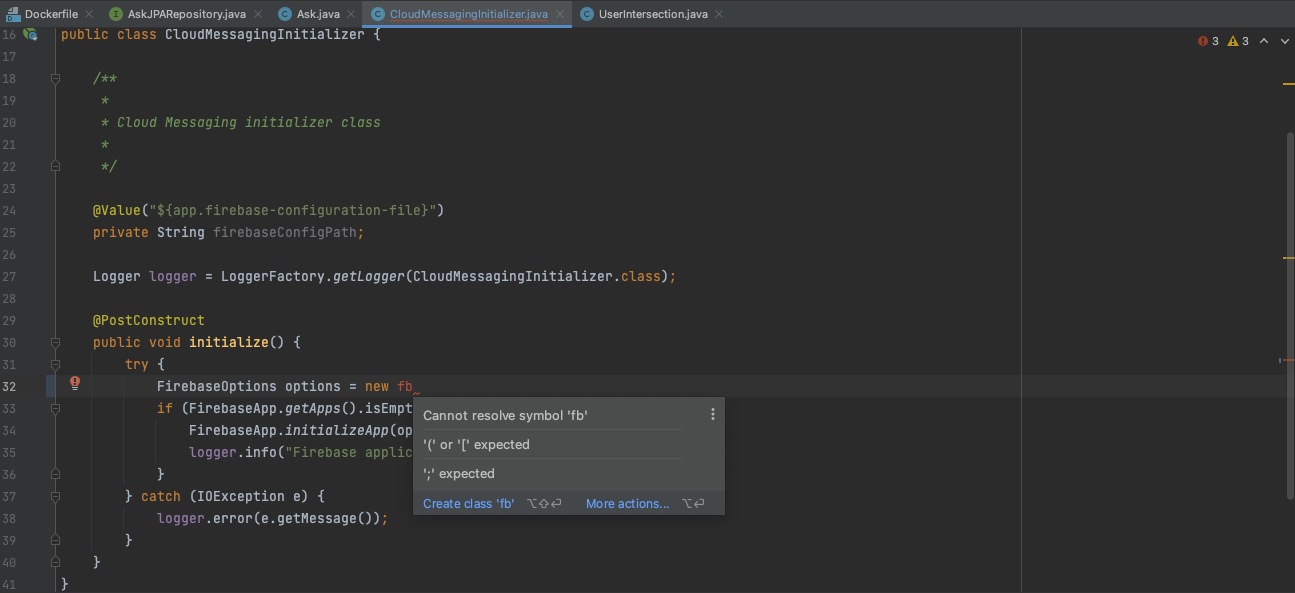
\includegraphics[width=\linewidth]{figs/token_unresolved.png}
  \caption{Unhelpful tooltip for syntax errors while typing in IntelliJ}
  \Description{Unhelpful tooltip for syntax errors while typing in IntelliJ}
\end{figure}
The following sections are dedicated to exploring each of these ideas in sufficient detail.

\subsection{Context based suggestions and Transformer based result ranking}
This proposal envisions enhancing with context based suggestions the tooltips currently displayed by IDEs on erroneous tokens, to aid the developer with faster error resolution. As illustrated in \textbf{Fig 1}, the tooltip only indicates that erroneous token can't be resolved, and which could possibly be enhanced with context based suggestions, such as either a constructor OR a builder instance, whichever is available for the current context; ie; \textit{'FirebaseOptions'} to help resolve the unresolved token \textit{'fb'}.
\newline
In order to do this, we would require a dependable token recommendation system which takes the current context into account. The most popular next token recommendation techniques utilize popular machine learning models such as Type-based inference or sequential Recurring Neural Network (SeqRNN) ones. However, as summarized comprehensively in \cite{FeedTree}, there exist major limitations in those two: Type-based models such as Jedi\footnote{https://github.com/davidhalter/jedi} or Eclipse\footnote{https://www.eclipse.org/pdt/help/html/working with code assist.htm} recommended and rank the next token in a very naive way (usually alphabetically), while their research has showed very clearly that popular machine learning based code prediction models such as SeqRNN recommends the next token in such a way that the correct result is present in approximately the top 2.7 results, leaving a definite margin for improvement.\cite{FeedTree}
\subsubsection{Transformer based intelligent next-token recommendation}
While the SeqRNN ML model yields impressive results in terms of next token recommendation, using Transformer-based models for next token prediction (instead of RNN) improved the ranking statistics: Correct results were displayed to developers within the first 1.5 - 2 results, an improvement of about 0.5 to 1 ranks higher.\cite{FeedTree}
\newline
A Transformer is a machine learning model first introduced by \textbf{GoogleBrain}.\footnote{https://research.google/teams/brain/} It is a type of model which processes input as a whole (for instance an entire sentence) and does not depend on past hidden states to retain past information (like Recurrent Neural Networks (RNN) do).\cite{vaswani2017attention} This has the advantage that Transformers don't risk losing past information.
\newline
An abstract syntax tree (AST) is generally defined as the abstract syntactic representation of source code.\cite{AST} Within this representation, each node of the AST represents a construct/token of the source code. The research in this paper postulates the above mentioned improvement in accuracy by feeding ASTs into Transformers. However, since Transformers are sequential models, only partial structures of the AST can be fed in at one point in time. Their solution to this was to explore three different methods to this end:\cite{FeedTree}
\begin{itemize}
    \item Decompose source code into partial programs and consequently each partial program into a sequential stream of source code tokens (SeqTrans)
    \item Decompose the AST into multiple paths and subsequently feed each path into the Transformer (PathTrans)
    \item Decompose the AST into its various traversal orders and subsequently feed each traversal into the Transformer (TravTrans)
\end{itemize}

\subsubsection{SeqTrans}
Since a Transformer is designed to take only sequential input, the input for this particular method works out of the box with the Transformer. A partial program (which is effectively a sequence of source code tokens) is fed as input to the Transformer, which in turn is expected to yield a single source code token as output.This method was already proven to be better than SeqRNN, as well as provided a platform for the following two AST based methods.
\subsubsection{PathTrans}
This method works on the concept of root paths: A root path is the path from a leaf node of an AST to to its root. Such an example is depicted in Fig 2
\begin{figure}[h]
  \centering
  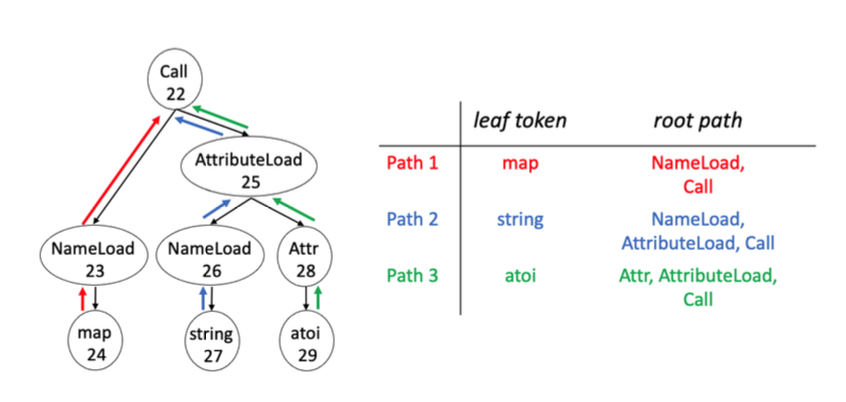
\includegraphics[width=\linewidth]{figs/rootpath.png}
  \caption{Rootpath concept}
  \Description{Example of leaf nodes in an AST and rootpaths to their root node}
\end{figure}
If an AST has multiple leaf nodes, there will be multiple root paths. Since each root path forms a sequence of internal nodes of the AST to each leaf token, it would ideally capture all the syntactical information along this path. Consequently, the root paths help in leaf token prediction when they are fed into the Transformer.
\subsubsection{TravTrans}
This method works on the concept of tree traversals;ie;feeding a sequence of nodes of the AST in a certain tree traversal order. The popular tree traversal methods include pre-order, post-order and in-order and can be applied to tree structures such as AST. The method involves feeding code token sequences which are obtained from pre-order traversals (in Depth First Search order since pre-order traversal is a kind of DFS) of the AST to optimize leaf token prediction.
\begin{figure}[h]
  \centering
  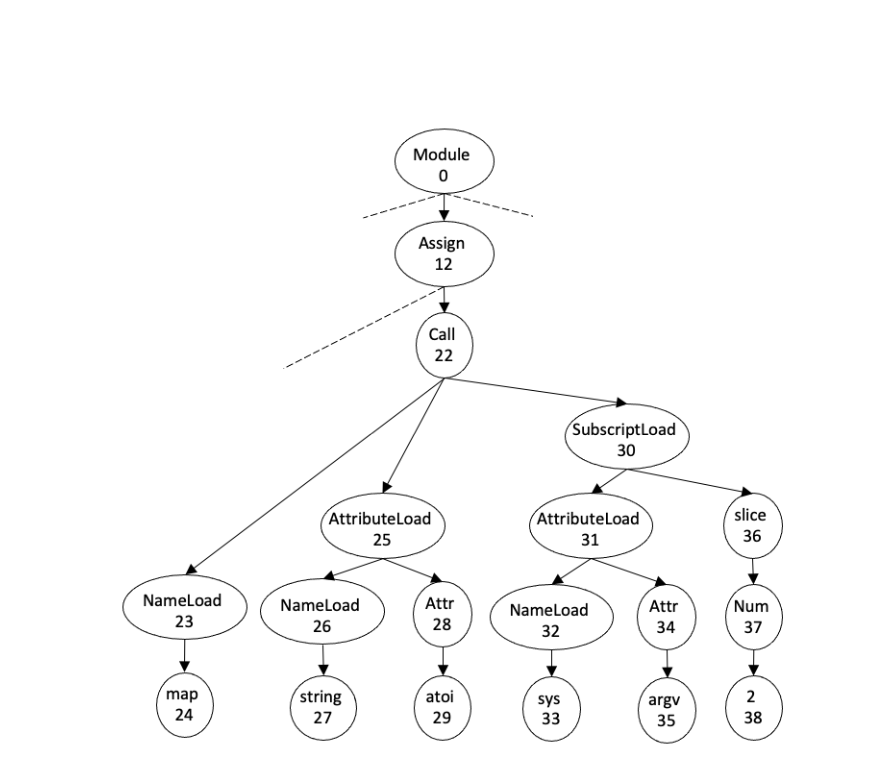
\includegraphics[width=\linewidth]{figs/dfs.png}
  \caption{AST as input to TravTrans}
  \Description{An AST which is decomposed is several token sequences through DFS}
\end{figure}
Fig 3 represents an AST. If we consider node 29 for example (atoi), the the node chain in DFS order preceding it would be:
\newline
\textbf{Call -> NameLoad -> Map -> AttributeLoad -> NameLoad -> string -> Attr}

\section{Envisioned implementation}
The token prediction results are generally expressed in terms of \textbf{mean reciprocal rank} percentages. As mentioned earlier, for typical RNN based methods, this percentage is about \textbf{37}, while the most efficient method, \textbf{TravTrans}, which functions on feeding AST tree traversal sequences to Transformers, was found to increase this percentage by about \textbf{18}. Since 37 roughly equates to the correct token being present in the first 2.7 results, this 18 percent increase meant that now the correct token could be present anywhere between the first 1.5 and 2 results. As a consequence, we propose to use TravTrans as the method of choice for input transformation. 
Meanwhile, similar to the implementation \cite{FeedTree}, this implementation would also require a large dataset. The dataset would comprise of source code files from any popular language (Java, Python etc.) decomposed into ASTs (to later be fed into Transformers). It follows logically that an increase in the size and variety of the dataset would serve to improve the accuracy of the recommendation. Since it could potentially be tested internal to a team or organization, the dataset could largely comprise of AST decomposed from internal source code repositories. Since it is generally inadvisable to reinvent the wheel and because it produce a proven increase in MRR (Mean Reciprocal Rank), we propose to opt for for the GPT-2 small implementation\cite{radford2019language} based on the PyTorch library\footnote{https://github.com/graykode/gpt-2-Pytorch}, similar to what was utilized in the research.\cite{FeedTree}. The schematic illustration of such a GP2 Transformer is depicted in Fig 4
\begin{figure}[h]
  \centering
  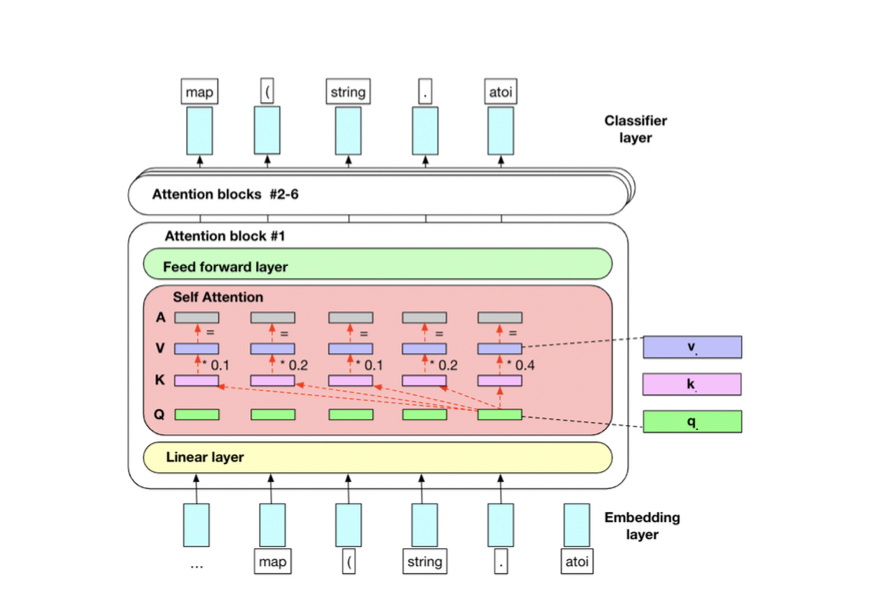
\includegraphics[width=\linewidth]{figs/transformer.png}
  \caption{GP2 Transformer}
  \Description{Schematic of a GP2 Transformer}
\end{figure}

% References
\bibliographystyle{ACM-Reference-Format}
\bibliography{references}

%%
%% If your work has an appendix, this is the place to put it.
%\section{Appendices}
%\appendix

%\section{My Appendix}
%
%Lorem ipsum

\end{document}
\endinput
